All of the details in \cref{chapter:qhl} and \cref{chapter:qmla} are implemented in the \gls{qmla}
    software framework, a (mostly) Python codebase which underlies all of the 
    arguments, results and figures in this thesis. 
The codebase is designed to simplify the process of running \gls{qmla} or \gls{qhl}
    on novel systems.
In particular, the core \gls{qmla} algorithm can support a wide range of \glspl{es}, 
    allowing for the design of bespoke \glspl{es} to account for the specific requirements 
    of any given system. 
In this chapter we give an overview of the \gls{qmla} software, 
    implementation and instructions for its use. 

\section{Implementation}
In this section we describe the technical details of the implementation of the 
    algorithm described in \cref{chapter:qmla}, as well as a number of relevant subroutines. 
We do not introduce new mathematical, physical or algorithmic concepts, 
    so readers interested in applications of the techniques may prefer to skip to \cref{part:theoretical_study}.

\subsection{Object oriented programming}
We first introduce the concepts of object-oriented programming, 
    and in particular \emph{inheritance} between objects, 
    since this will feature in later discussion about the implementation of \gls{qmla}
    and \glspl{es}. 
Python is a robust object-oriented language \cite{python-manual}, meaning that we can frame 
    concepts as objects which permit actions to be performed by/to them. 
In particular, objects in Python are formulated as \emph{classes}, 
    which can have associated \emph{attributes} and \emph{methods}. 
For example, we can encode the concept of a footballer as an object,
    such that the player object has attributes, e.g. number of games played and goals scored in a season, 
    as well as methods for specific calculations, 
    e.g. to summarise their record.
We can then utilise the footballer class to store information about an \emph{individual} player, 
    by making an instance of the class.
\par 

A fundamental concept in object-oriented programming is \emph{inheritance} between objects, 
    such that a \emph{child} objects inherit properties of its \emph{parent}.
In general, a parent object can be thought of as an abstract concept, 
    which provides basic functionality and reasonable default properties,
    while a child object can specify further details. 
For example, an Athlete class can act as a parent to the footballer class, 
    where the Athlete class holds core information such as date of birth. 
This allows for the Athlete class to be recycled as the \emph{base} class for other child classes
    which have the same underlying requirements, e.g RubgyPlayer. 
We list this example in \crefrange*{listing:athlete_class}{listing:footballer_class}. 

\begin{lstlisting}[
    label=listing:athlete_class,
    caption={Parent class, encoding the concept of an athlete.}
]
class Athlete():
    
    def __init__(
        self, 
        name, 
        birth_day, 
        birth_month, 
        birth_year, 
    ):
        # Use information given
        self.name = name
        self.date_of_birth = datetime.date(
            birth_year, birth_month, birth_day
        )
        
    def age(self, round_down=True):
        days_since_birth = datetime.date.today() - self.date_of_birth
        age = days_since_birth.days / 365
        
        if round_down:
            age = int(age)
        
        return age
    
    def summary(self):
        summary = "{name} is a {age}-year old athlete.".format(
            name = self.name, 
            age = self.age()
        )
        print(summary)
        
        
bob = Athlete(
    name='Bob',
    birth_day = 11,
    birth_month = 11, 
    birth_year = 1993, 
)
bob.summary()    
\end{lstlisting}

\begin{lstlisting}[
    label=listing:footballer_class,
    caption={Child class, encoding the concept of a footballer, which adopts the abstrat representation of an athlete.}
]
class Footballer(Athlete):
    def __init__(
        self, 
        footed,
        team, 
        size = 'medium',
        **kwargs
    ):
        # Pass arguments to the parent class
        super().__init__(**kwargs)
        
        # Use information given
        self.team = team
        self.footed = footed
        self.size = size
        
        # Default attributes
        self.goals_scored = 0 

    def summarise(self):
        summary = "{size} {player} plays for {team} and has scored {num_goals} goals.".format(
            size = self.size, 
            player = self.name, 
            team = self.team, 
            num_goals = self.goals_scored
        )
        print(summary)
        
    def record_goals(self, num_new_goals):
        self.goals_scored += num_new_goals
        
        
mickey = Footballer(
    name = 'Mickey', 
    footed = 'left',
    team = 'QECDT-FC',
    birth_day = 1,
    birth_month = 1, 
    birth_year = 1990,
    size = 'Big'
)
mickey.record_goals(num_new_goals = 10)
mickey.summarise()    
\end{lstlisting}

\section{Python framework}
\begin{figure}
    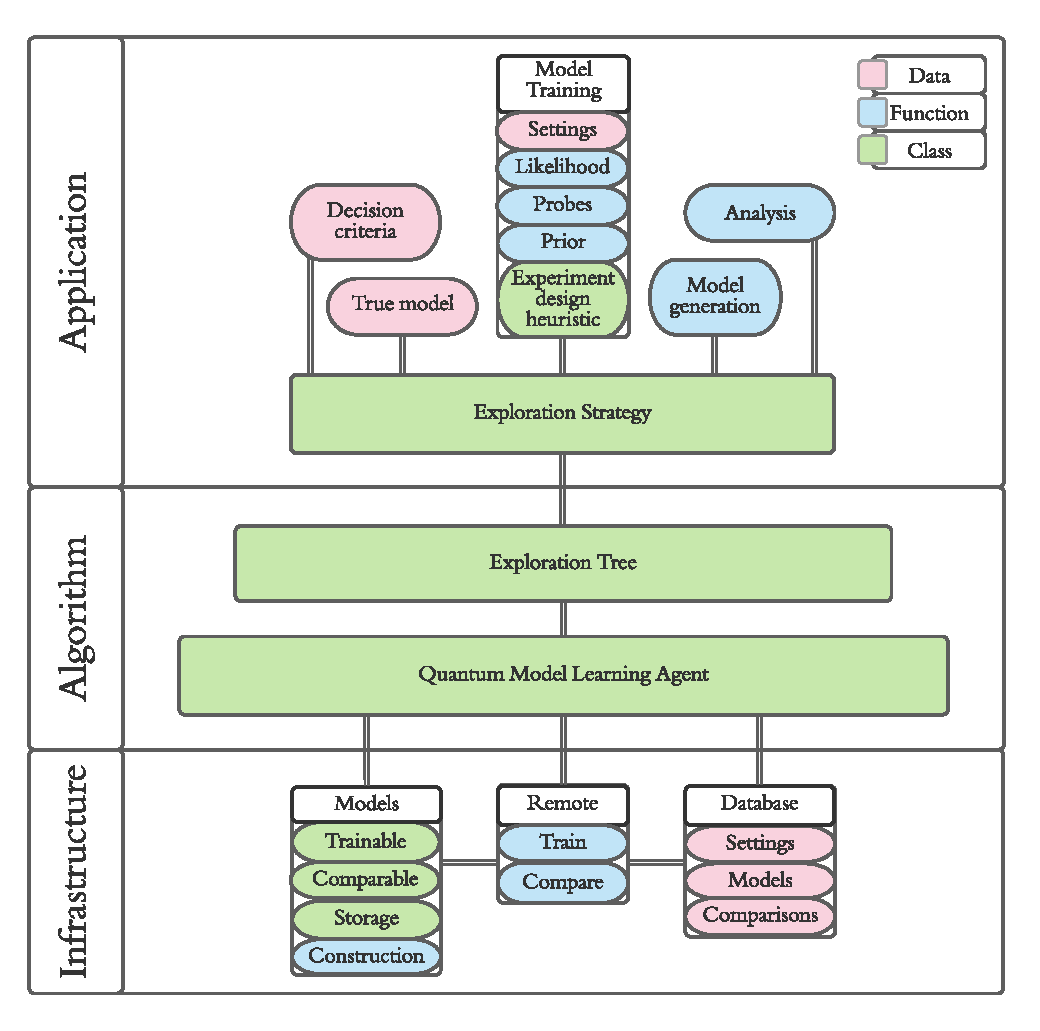
\includegraphics{algorithms/figures/software_overview.pdf}
    \caption[ \Glsentrylong{qmla} codebase overview]{
        Overview of important \emph{objects} in the \gls{qmla} framework.
        Colours encdoe the type of object: red objects are \emph{data}, blue are \emph{functions/methods} 
        and green are \emph{classes}. 
        Objects are grouped broady, with double lines showing communication channels between (groups of) objects. 
        \emph{Infrastructure}: functions for the implementation of model training/comparisons on 
        a remote server.
        \emph{Algorithm}: implementation of the iterative procedures and decision-making 
        laid out in \cref{chapter:qmla}. 
        \emph{Application}: inter-changeable data/functionality for the unique requirements 
        of a given target system. 
        Users wishing to customise \gls{qmla} must choose a valid object for each of those in \emph{applications}, 
            and need not alter any of the underlying framework.
    }
    \label{fig:software_overview}
\end{figure}

A driving motivation for the development of \gls{qmla} is generality:
    we endevaour to make \gls{qmla} applicable to any target quantum system.
We provide a framework, where users can tailor the inputs and methodology to their needs:
    we depict the main components of the framework in \cref{fig:software_overview}, 
    broadly grouping concepts as part of its \emph{infrastructure}, \emph{algorithm}
    or \emph{application}. 
In short, users need only specify the elements of the framework in the \emph{application} segment, 
    without concern for the underlying mechanics of \gls{qmla}; 
    in particular, users interface with the framework through the design of a bespoke \gls{es}, described next. 


\subsection{Application}\label{sec:application}
The application of \gls{qmla} refers to the choice of target system, \gls{q}, and how \gls{qmla} searches the 
     \gls{model search}  in attempt to discover its model. 
As outlined in \cref{sec:exploration_strategies}, \glspl{es} play the role of 
    defining \gls{qmla}'s objectives, guiding the steps it takes, and designing the models to be tested. 
We facilitate the study of any system by providing a robust \ttt{ExplorationStrategy} base class,
    with all of the functionality expected of a generic \gls{es}, allowing users to inherit and build upon it. 
In particular, \glspl{es} allow users to specify the implementation of aspects listed in \cref{sec:exploration_strategies}, 
    as well as further details.
\par 


\subsubsection{Modular functionality}\label{sec:modular_functionality}
The most crucial methods\footnotemark \ of the \gls{es} class are modular, 
    described in \cref{sec:modular_functionality},
    meaning that they can be directly replaced, provided the alternative method fulfils the same role. 
Our base \gls{es} class uses sensbile defaults for this modular functionality, 
    but this flexible mechanism allows for adapting \gls{qmla} by choosing an approach for each 
    of the following subroutines. 
\footnotetext{
    The words \emph{method} and \emph{function} are mostly interchangeable, although methods are specifically associated with a class, 
    while functions are stand-alone.
}

\begin{easylist}[itemize]
    & \gls{likelihood} function. By default, \gls{qhl} calls a subroutine to compute \cref{eqn:likelihood}. 
        This can be replaced by any function which, given a Hamiltonian, evolution time and \gls{probe} state, 
        returns the likelihood, according to the experiment you wish to simulate. 
        For example, in \cref{chapter:nv}, the data on which models are trained comes from experimental measurements, 
            so we replace the\gls{likelihood} function with a calculation corresponding to the experimental procedure. 
        Importantly, QInfer requires the quantity $\Pr(0)$, see \cref{eqn:pr0}, so that is the output of these functions. 
    & \Gls{probe} generation. The training phase requires a set of probes against which to optimise individual models. 
        Users may wish to specify the design of such probes, for example to match experimental constraints 
        which restrict the realisible probes in the performance of the experiment. 
        Alternatively, it may be feasible to design probes which increase the information gained per experiment, 
        enabling faster learning. 
    & \Glsentryfull{edh}. The choice of \gls{edh} greatly influences how the training will perform. 
        We provide a base class implementing \gls{pgh}, as well as child classes for each of 
        the \glspl{edh} listed in \cref{sec:alt_heuristics}. 
    & Prior. The method of drawing the prior distribution can be replaced, for example, with 
        a method for constructing a uniform distribution on each parameter.
        A key input to the procedure is the initial knowledge the user has about the system, 
        which is encoded in the prior, for instance varying orders of magnitude of the viable terms.
\end{easylist}

Additionally, applications require a series of settings for the model training phase, 
    such as the \glspl{hyperparameter} required by the resampling algorithm, \cite{liu2001combined}, 
    as well as detailing the true (target) model, $\ho$, in the case where \gls{q} is a simulated quantum system.
We can also specify some \gls{es}-specific analyses to examine its internal performance, 
    although this is generally required during development/testing, and less useful thereafter. 

\subsection{Algorithm}\label{sec:sw_algorithm}
The algorithm layer of \cref{fig:software_overview} implements the core steps of \gls{qmla},
    as shown in \cref{fig:qmla_overview}, by running a set of \glsentryfullpl{et}, 
    each of which communicate with a unique \gls{es}. 
The core \gls{qmla} class manages the database of models and their comparisons,
    and decides how to react at certain stages, by consulting the decision criteria set by the \gls{es}. 
\par 

\subsubsection{Parallel implementiation}\label{sec:parallel}
\begin{figure}
    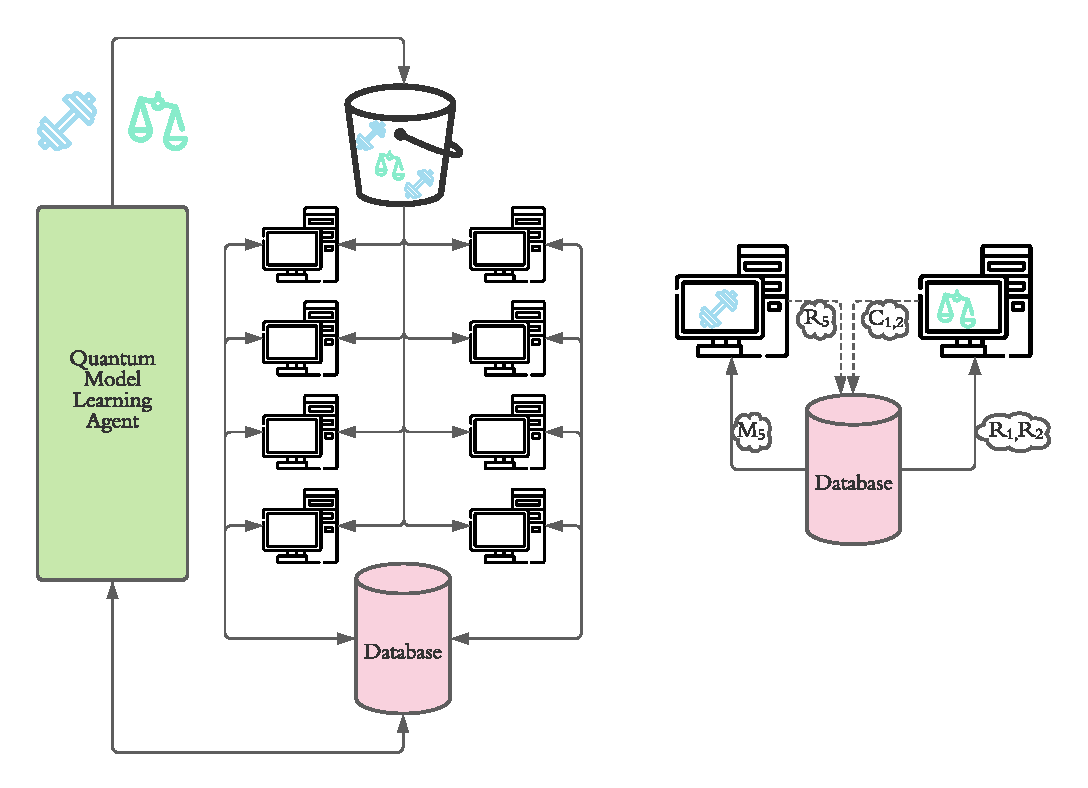
\includegraphics{algorithms/figures/parallel_architecture.pdf}
    \caption[Parallel architecture for \gls{qmla}]{
        Parallel architecture for \gls{qmla}.
        \textbf{Left}, \gls{qmla} generates tasks 
            -- either to train (blue dumbbells) or compare (oragne scales) models -- 
            and places them in a task queue. 
        Worker processes (depicted as computers) retrieve those tasks and compute them in parallel, 
            and interact with a database. 
        \textbf{Right}, Distributed tasks occuring in parallel. 
        The left-hand process assumes the task of training the model with ID 5:
            it first queries the database for a packet of core information, $M_5$, 
            which informs the model training procedure, for example the terms and parameters 
            of model 5. 
        After training, it sends a packet, $R_5$, summarising the result of model 5's training. 
        The right-hand process compares two models with IDs 1 and 2, by first retrieivng the results packets
            $R_1, R_2$, then storing the comparison $C_{1,2}$ on the database. 
    }
    \label{fig:parallel}
\end{figure}

The implementation of \gls{qmla} seeks to separate the organisation of the  \gls{model search}  from the 
    cumbersome calculations which enable the search. 
We can offload those calculations to a compute cluster (server) to run \emph{in parallel},
    allowing for significant speedup of the entire \gls{qmla} procedure, 
    limited by Amdahl's law. % TODO reference/explain Amdahls law (do we need it here? somewhere else?) 
\gls{qmla} distributes jobs to \emph{worker} processes in a server, 
    i.e. we assume that \gls{qmla} is run on a machine with $N_c$ available parallel \emph{processes}\footnotemark. 
Then, the expensive calculations, namely training and comparing models, are not performed 
    directly within the \gls{qmla} class, but instead are farmed out across the server.
The role of \gls{qmla} then is to collate the outcome of those calculations in conjunction with the set of \glspl{et}, 
    until each \gls{et} is deemed complete, and then to consolidate the set of 
    \gls{et} champions, ultimately setting the global champion, $\hp$. 
Thereafter it can perform some analysis, e.g. to generate a series of plots which demonstrate how the 
    model search progressed, as well as the evidence in favour of $\hp$, including for example 
    the reproduction of \gls{q}'s dynamics by $\hp$. 
See \cref{sec:qmla_analysis} for further details. 

\footnotetext{Note when running in \emph{serial} (e.g. running locally on a personal machine), it is valid to simply set $N_c=1$.}
\par 

While there are a number of strategies for parallelising code over a cluster, 
    we use the \emph{master-worker} strategy, where one process acts as the \emph{master}, 
    determining which calculations are required at any given moment, 
    then brokering self-contained tasks to \emph{workers}, 
    which blindly solve a small problem, without knowledge of the wider context or algorithm \cite{hockney2019parallel}.
The mapping here is trivial: the master of our algorithm is \gls{qmla}, 
    while workers can be used for the tasks of training and comparing models. 
The \gls{qmla} class is hence assigned a single process solely for its considerations, 
    e.g. for the ranking of models and determination of the next models to tests, 
    while the remaining $N_c - 1$ processes lay dormant until \gls{qmla} requests that they perform a job. 

\par 
We use a simple \emph{task queue} for the distribution of jobs: 
    \gls{qmla} adds tasks to the queue and any available worker can take the next job and compute it. 
There are two types of task for workers:
\begin{easylist}
    & to train a candidate model $\hi$:
        the worker first requests some essenital information about the model from the databse, 
        e.g. the name, terms and prior associated with the model, packaged in $M_i$;
        following completion, the worker compresses the result, $R_i$, and sends it to the database for storage. 
    & to compare two models, $\hi, \hj$: 
        the worker retrieves $R_i, R_j$ from the database, performs the calculation, 
        and returns the compressed outcome of the comparison, $C_{ij}$, to the database. 
\end{easylist}
The master \gls{qmla} class can also access said database, and copies the compressed results packets $R_i$ and $C_{ij}$,
    in order to account for the results in its decision-making. 
It is worth noting that tasks are completely independent, so some worker processes
    may compute comparisons while others train models simultaneously, 
    although obviously the comparison can not begin until both $R_i, R_j$ are available. 
This is dealt with easily by using a \emph{blocking} protocol, 
    where new batches of jobs are not released until the master receives all the results of jobs on which the new tasks depend.
\gls{qmla} simply waits until all models on a given layer have been trained before queueing comparisons 
    on that layer, to ensure a comparison can not start without the data needed to compute that comparison. 
\par

Models are assigned a unique ID upon creation; 
    models are uniquely described by their name, represented as a string in the \gls{qmla} class, 
    such that newly proposed models can be checked against the set of previously considered models 
    before being added to the database. 
\gls{qmla} can hence check whether a proposed model has already been trained, 
    in which case it does not resubmit the model, but instead relies on the previous result. 
Likewise \gls{qmla} can check for the presence of any comparison result $C_{ij}$ before setting it as a new task, 
    ensuring we do not duplicate expensive calculation. 
\par 
We use a redis database and task queue \cite{redis, redis_queue}. 
We depict the structure of this parallel architecture, and the master-worker strategy, in \cref{fig:parallel}.

\subsection{Infrastructure}\label{sec:infrastructure}
The infrastructure enabling the distribution of \gls{qmla}'s tasks across 
    a set of worker processes can be summarised as
\begin{easylist}
    & a set of classes representing the objects on which we must perform expensive calculations;
    & functions to launch those calculations independently of any other calculation;
    & a database which can be accessed by all workers as well as \gls{qmla}.
\end{easylist}
\par 

We need a series of distinct classes to represent models, for use in each stage of \gls{qmla}: 
    a \emph{trainable} class is used for the parameter optimisation, 
    while \emph{comparable} classes are used for computing \glspl{bf}, 
Crucially, this separation allows us to perform data-heavy calculations independently, 
    e.g. on a remote process within a compute cluster, 
    and discard the class instance used for the calculation and the large amount of data it generates, 
    while only the relatively small \emph{storage} classs is retained by \gls{qmla} for later use. 

\par 
The tasks which actually implement the calculations (\cref{sec:parallel}) are captured by standalone \emph{remote} functions. 
These functions receive instructions such as \ttt{train model 10}; 
    they then contact the database for the set of shared settings, 
    such as $\Ne, \Np$ and the set of probes, 
    before performing the task, and then sending the compressed result to the database for storage. 

\par 
To achieve this separation between calculation and analysis, we use a redis database \cite{redis},
    which holds the core implementation settings, e.g. $\Ne, \Np$ and the set of probes to train upon, 
    as well as the compressed summaries of the outcomes of tasks

\section{Usage}

Several aspects of \gls{qmla} are \emph{probabilistic}.
Firstly, the Bayesian updates within model training of \gls{qhl} relies on \glspl{likelihood}  which 
    implicitly depend on the measurement datum of a quantum system; 
    in the case where the the measurement collapses \gls{q} into the less-likely basis, 
    the \glspl{likelihood}  will reflect that accurate hypotheses were poor, 
    resulting in misguided posterior distributions. 
It is thus \emph{possible} that the parameter learning will converge on incorrect values. 
Moreover, the model design subroutine is not gauranteed to exploit the aspects of favoured models which are 
    actually informative, e.g. given a favoured model with four correct terms and two incorrect terms, 
    the model generator may opt to build on the incorrect terms, in the common situation where it does not know 
    which constituent terms are helpful and which aren't. 
\par 
Overall, then, it is pertinent to run \gls{qmla} many times and gather statistics about its performance, 
    rather than making overly-strong claims about \gls{q} based on a single \emph{instance} of the algorithm. 
We say that a \gls{qmla} \emph{\gls{run}} consists of $N_r$ independent \emph{\glspl{instance}},
    which can be run in parallel, such that we are primarily concerned with the performance of the run 
    instead of any individual instance. 
For example, with $N_r=100$, we can interpret the \emph{ \gls{win rate} } of every model in the model space
    as evidence for that model being $\ho$.
For the sake of evaluating \gls{qmla} itself, as in \cref{part:theoretical_study}, 
    we can use the  \gls{win rate}  of $\ho$ as indication of the \emph{\gls{success rate}}, 
    i.e. the fraction of \glspl{instance} within a run where \gls{qmla} identifies precisely $\hp = \ho$. 
Note, however, that neither the  \gls{win rate}  nor \gls{success rate} are singularly informative 
    of \gls{qmla}'s performance: in some cases, we can deem \gls{qmla} successful even if it does not 
    identify $\ho$ exactly, e.g. if it finds the majority of terms present in $\termset_0$ from a large space, 
    i.e. a high $\fs$, see \cref{sec:f_score}. 


\subsection{Outputs and analysis}
When a \gls{run} is launched, \gls{qmla} generates a \emph{\gls{results directory}} unique to that \gls{run}, 
    identified by the time and date of its launch,
    in which all the pertinent information for that \gls{run}, including raw data and figures, are stored. 
It includes an \ttt{analyse.sh} script to generate analysis after all \glspl{instance} have completed\footnotemark. 
\gls{qmla} provides a large amount of anaytics to assess the performance of the protocol. 
These range from \emph{big picture} perspectives such as the  \gls{win rate}  across the entire \gls{run}, 
    to zooming in on the internal metrics for training individual models.
Some of these analyses are generated by default, while others are optional depending on the 
    level of detail the user requires. 
A number of sub-directories are produced in the \gls{results directory}, 
    each containing data/figures from a different view of the \gls{run};
    these are listed in \cref{apdx:figure_repoduction}.
\footnotetext{
    Note this script is not run automatically since, on remote servers, \glspl{instance} finish independently without any central process
    noticing. Therefore this script must be run by the user when the run is complete.
}
\par 

The user has control on which plots are generated, in order that the appropriate level of degree is 
    presented, without producing an excessive number of images which can slow the protocol down. 
Results are categorised across the levels of the framework, defined as:
\begin{description}
    \item[\Gls{run}]: results across a number of instances.
    \begin{easylist}
        && the number of \gls{instance} wins for \glspl{champion model}.
        && average dynamics reproduced by \glspl{champion model}.
    \end{easylist}
    
    \item[\Gls{instance}] performance of a single insance.
    \begin{easylist}
        && models generated and the branches on which they reside
    \end{easylist}

    \item{\Gls{model}] Individual model performance within an instance.
    \begin{easylist}
        && parameter estimation through QHL.
    \end{easylist}

    \item[Pairwise Comparisons] direct comparison of models’ performance.
    \begin{easylist}
        && dynamics of both candidates (with respect to a single basis).
    \end{easylist}

    \item[\Glsentrylong{es}] figures specific to the \gls{es}
    \begin{easylist}
        && model generation metrics
    \end{easylist}
\end{description}
\par 

Most plots used in this thesis are generated directly by the \gls{qmla} framework\footnotemark; 
    the \gls{es} class and implementation parameters of each figure is listed in \cref{table:figure_reproduction}.
\footnotetext{Or are minor modifications of auto-generated plots.}
